\chapter{Modelado analítico de la PCC \label{chap:ModeloPCC}}
\noindent Además de los sesgos que añaden el fondo y el umbral utilizado sobre la determinación de las magnitudes del factor de Fano y la energía de creación electrón-hueco, la colección parcial de carga juega un rol fundamental en la determinación precisa de estas magnitudes. Como se verá en este capítulo el efecto de este fenómeno resulta particularmente apreciable para las mediciones realizadas con los rayos $X$ emitidos por el flúor y aluminio, por ser su energía significativamente menor que la emitida por los $X$ del $^{55}$Fe estudiado en trabajos previos\cite{TesisAndi,TesisKevin,Rodrigues}.

%%%%%%%%%%%%%%%%%%%%%%%%%%%%%%%%%%%%%%%%%%%%%%%%%%%%%%%%%%%%%%%%%%
%%%%%%%%%%%%%%%%%%%%%%%%%%%%%%%%%%%%%%%%%%%%%%%%%%%%%%%%%%%%%%%%%%
\section{Introducción del modelo}
\noindent La física detrás de los fenómenos de colección parcial de carga y eficiencia de colección de carga puede comenzar a modelarse estudiando la distancia que recorren los fotones dentro del material del sensor hasta que interactúan con él. Esta es una variable aleatoria con distribución exponencial, por lo tanto, su función densidad de probabilidad es:
\begin{equation}
    f_{Z}(z) = \frac{1}{\tau_{\scaleto{X}{4pt}}}\exp(-\frac{z}{\tau_{\scaleto{X}{4pt}}})
        \label{ec:DistribucionDistancias}
\end{equation}
donde $\tau_{\scaleto{X}{4pt}}$ es la longitud de atenuación, es decir, la distancia promedio para la cual la cantidad de fotones incidentes se reduce a una fracción de $1/e$ de la población original. Este es un valor tabulado que depende tanto de la energía de los fotones como del material. Para el caso del silicio, puede verse en el gráfico de la Figura \ref{fig:Attenuation} la relación entre la longitud de atenuación $\tau_{\scaleto{X}{4pt}}$ y la energía de un fotón incidente. Por ejemplo, para el caso de la energía correspondiente a los rayos $X$ del flúor, $677\,\si{eV}$, se tiene que la longitud de atenuación es aproximadamente $1\,\si{\mu m}$, mientras que para los rayos $X$ del aluminio, $1486\,\si{eV}$, la longitud de atenuación ronda los $8\,\si{\mu m}$.
\begin{figure}[h]
    \centering
        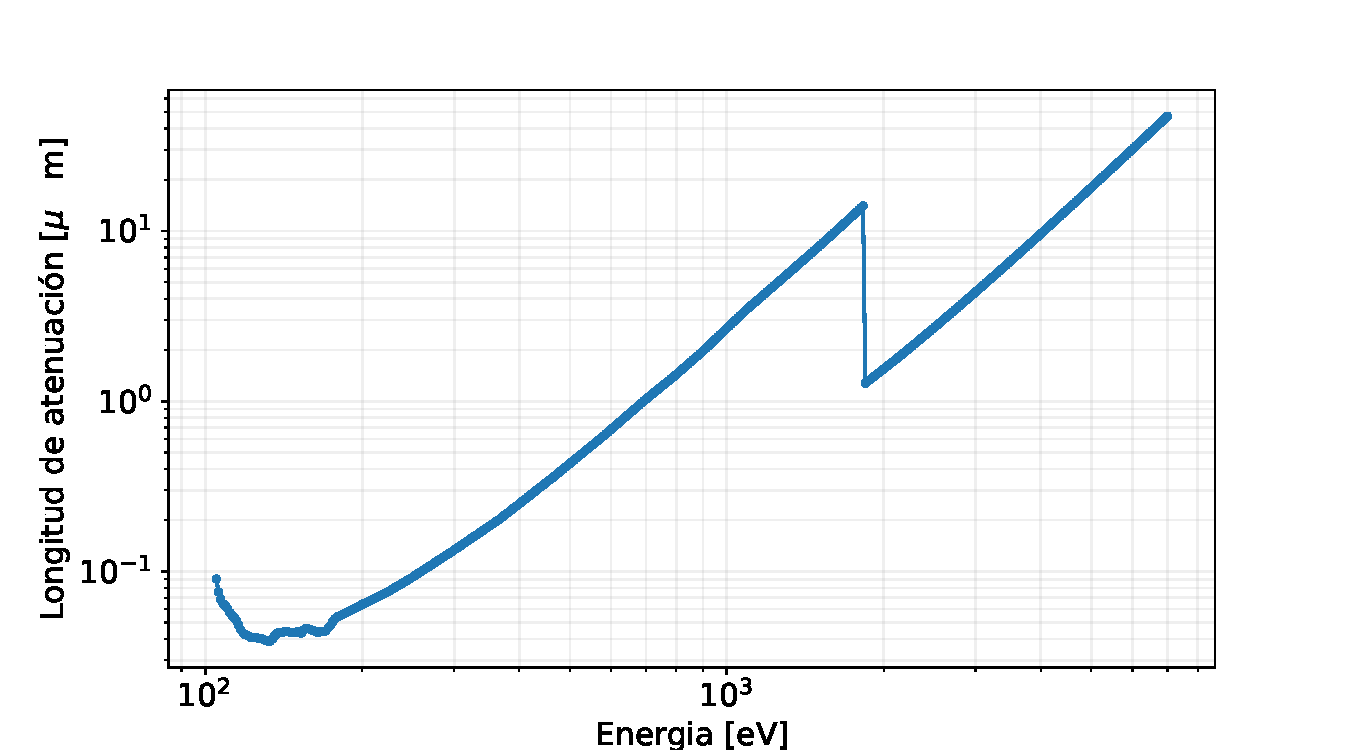
\includegraphics[scale=0.5]{Figs/AttenuationLength.pdf}
    \caption{\footnotesize{Longitud de atenuación para el silicio en función de la energía de un fotón que incide con un ángulo de $90\,^{\circ}$ sobre el material. Datos obtenidos de \textit{The Center for X-Ray Optics}\cite{AttenuationLength}.}}
    \label{fig:Attenuation}
\end{figure}
Realizaciones de la variable aleatoria que sigue esta distribución son las diferentes distancias que puede alcanzar un fotón que penetra en el sensor hasta generar cargas por ionización.

Por otro lado, se puede caracterizar la eficiencia de colección de carga con una función para la cual a una dada distancia de penetración $z$ se tiene qué fracción de la carga inicial logra ser colectada. Dicha función viene dada por
\begin{equation}
    E_{ff}(z) = 1 - 
    \exp
    \left(
        -\frac{z}{\tau_{\scaleto{CCE}{4pt}}}
    \right)
        \label{ec:funcionCCE}
\end{equation}
donde $\tau_{\scaleto{CCE}{4pt}}$ es la distancia media para la cual la cantidad de carga ionizada que sufre recombinación cae a $1/e$ del total de carga inicial. En el gráfico de la Figura \ref{fig:EficienciaCC} se presentan los datos obtenidos de practicar el análisis propuesto Moroni et al.\cite{PCC-CCE-interno} sobre las mediciones obtenidas con los rayos $X$ del F y su ajuste a partir del uso de esta función. De este ajuste se obtiene un valor $\tau_{\scaleto{CCE}{4pt}} = (0.0914 \pm 0.0027)\,\si{\mu m} $ para el cual la cantidad de carga que sufre recombinación cae a una fracción $1/e$ de la cantidad de carga inicial.
\begin{figure}[h]
    \centering
        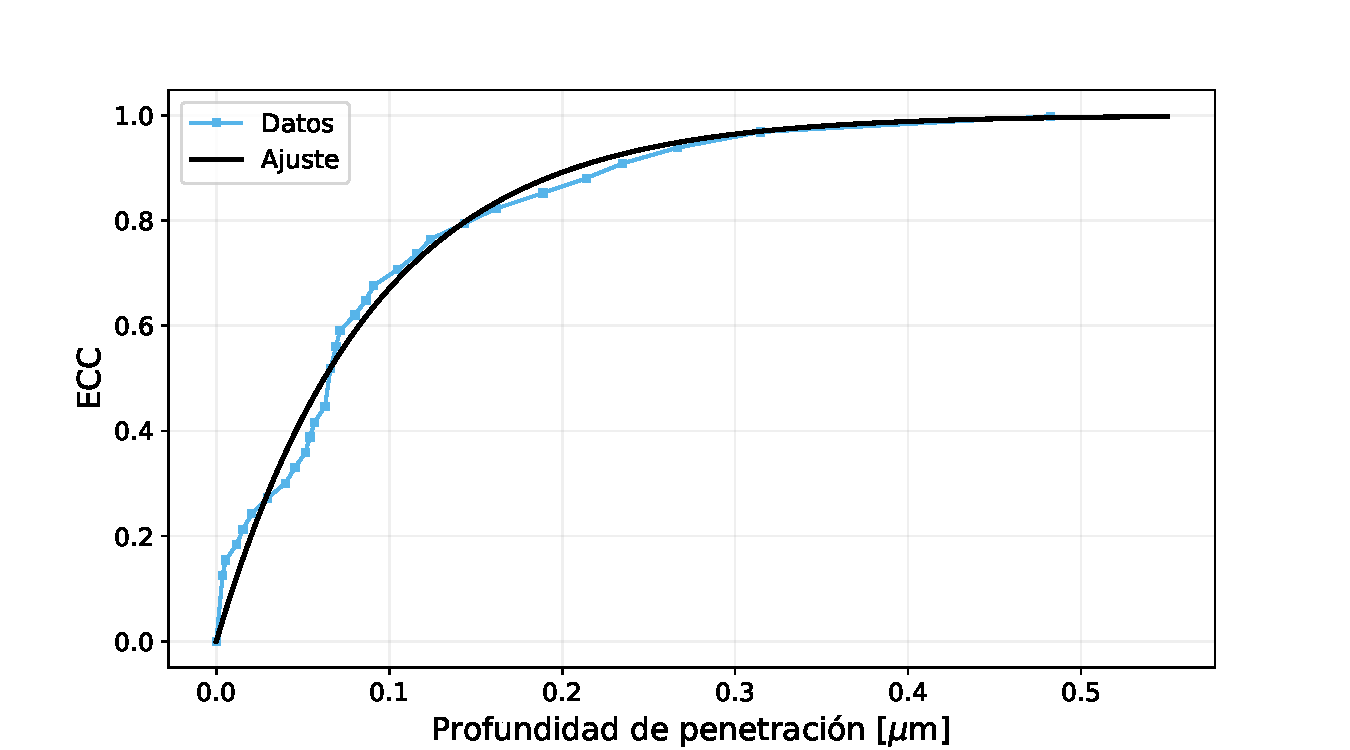
\includegraphics[scale=0.5]{Figs/CCE_vs_z.pdf}
    \caption{Mediciones de la eficiencia de colección de carga como función de la profundidad y ajuste de los mismos utilizando la función de eficiencia de la colección de carga. Datos obtenidos de mediciones con rayos $X$ del flúor de $677\,\si{eV}$. Del ajuste se obtiene $\tau_{\scaleto{CCE}{3pt}} = (0.0914 \pm 0,0027)\,\si{\mu m} $. Se ve que luego de los primeros $100\,\si{nm}$ logra colectarse cerca del $65\,\%$ de carga y como luego de los primeros $\sim 400\,\si{nm}$ ya es colectada casi el $100\,\%$ de la carga producida por ionización.}
    \label{fig:EficienciaCC}
\end{figure}
Esta cantidad, $\tau_{\scaleto{CCE}{4pt}}$ representa el ancho efectivo de la región de colección parcial de carga del detector.% de forma que obteniendo $\beta$ a partir del ajuste y $\tau_{\scaleto{X}{4pt}}$ a partir de tablas, se puede saber el tamaño efectivo de la región de PCC. %De acuerdo al gráfico de la Figura \ref{fig:EficienciaCC}, para mediciones tomadas a partir de rayos $X$ de $677\,\si{eV}$, se ve que luego de los primeros $100\,\si{nm}$ ya logra recuperarse más del $65\,\%$ de la carga ionizada, es decir, la cantidad de carga que sufre recombinación cae a $\sim 1/e$ de la cantidad total. De aquí puede decirse que en este caso $\tau_{\scaleto{CCE}{4pt}} \approx 0.1\,\si{\mu m}$ con lo cual este es el ancho de la región de PCC del sensor, de acuerdo a esta definición.

Se busca combinar ambas expresiones, donde la primera de ellas es una distribución y describe un proceso estocástico mientras que la segunda es una función convencional. Para esto es necesario lograr incorporar la variable aleatoria $z$, que viene de la función densidad de probabilidad \ref{ec:DistribucionDistancias}, dentro de la función de eficiencia \ref{ec:funcionCCE}, de modo de obtener una nueva función densidad de probabilidad $f_{E_{ff}}$ para la variable aleatoria \textit{eficiencia} o \textit{probabilidad de colectar carga}, que representaremos con la letra griega $\varepsilon$. La nueva variable aleatoria $\varepsilon$ tiene una dependencia funcional conocida con la variable aleatoria $z$ y viene definida por $\varepsilon = E_{ff}(z)$. En este sentido, dada una correspondencia uno a uno entre la vieja y la nueva variable, la probabilidad en un intervalo diferencial tiene que conservarse, con lo cual, dada la función densidad de probabilidad $f_{Z}(z)$ inicial y la función densidad de probabilidad final $f_{E_{ff}}(\varepsilon)$, tiene que valer que
\begin{equation*}
    f_{Z}(z)\,dz = f_{E_{ff}}(\varepsilon)\,d\varepsilon
\end{equation*}
de esta forma se puede escribir $f_{E_{ff}}$ en términos de la función densidad de probabilidad inicial como sigue
\begin{equation*}
    f_{E_{ff}} 
    = f_{Z}
    \left|
        \frac{dz}{d\varepsilon}
    \right|
\end{equation*}
donde aparece un Jacobiano y se agrega el módulo para asegurar una dependencia no negativa. Como la nueva variable aleatoria $\varepsilon$ es función de $z$, $E_{ff}(z) = \varepsilon$, entonces $E_{ff}^{-1}(\varepsilon) = z$ y se puede escribir la última en términos de $\varepsilon$
\begin{equation*}
    f_{E_{ff}}(\varepsilon) 
    = f_{Z}
    \left(
        E_{ff}^{-1}(\varepsilon)
    \right)
    \left|
        \frac{dE_{ff}^{-1}(\varepsilon)}{d\varepsilon}
    \right|
\end{equation*}
finalmente, resolviendo esta última se obtiene la expresión para la nueva función densidad de probabilidad, que resulta ser una Beta de parámetro $\alpha = 1$ y $\beta$ libre.
\begin{equation*}
    f_{E_{ff}}(\varepsilon) = \beta (1 - \varepsilon)^{\beta - 1}
\end{equation*}
donde además se definió el parámetro $\beta$ como $\beta = \frac{\tau_{\scaleto{CCE}{3pt}}}{\tau_{\scaleto{X}{3pt}}}$. 
Esta es la función densidad de probabilidad de colectar la carga producida por un fotón de una dada energía y puede verse un ejemplo de ajuste a un conjunto de datos simulados con esta distribución en la Figura \ref{fig:BetaDistyAjuste}.
\begin{figure}[h]
    \centering
        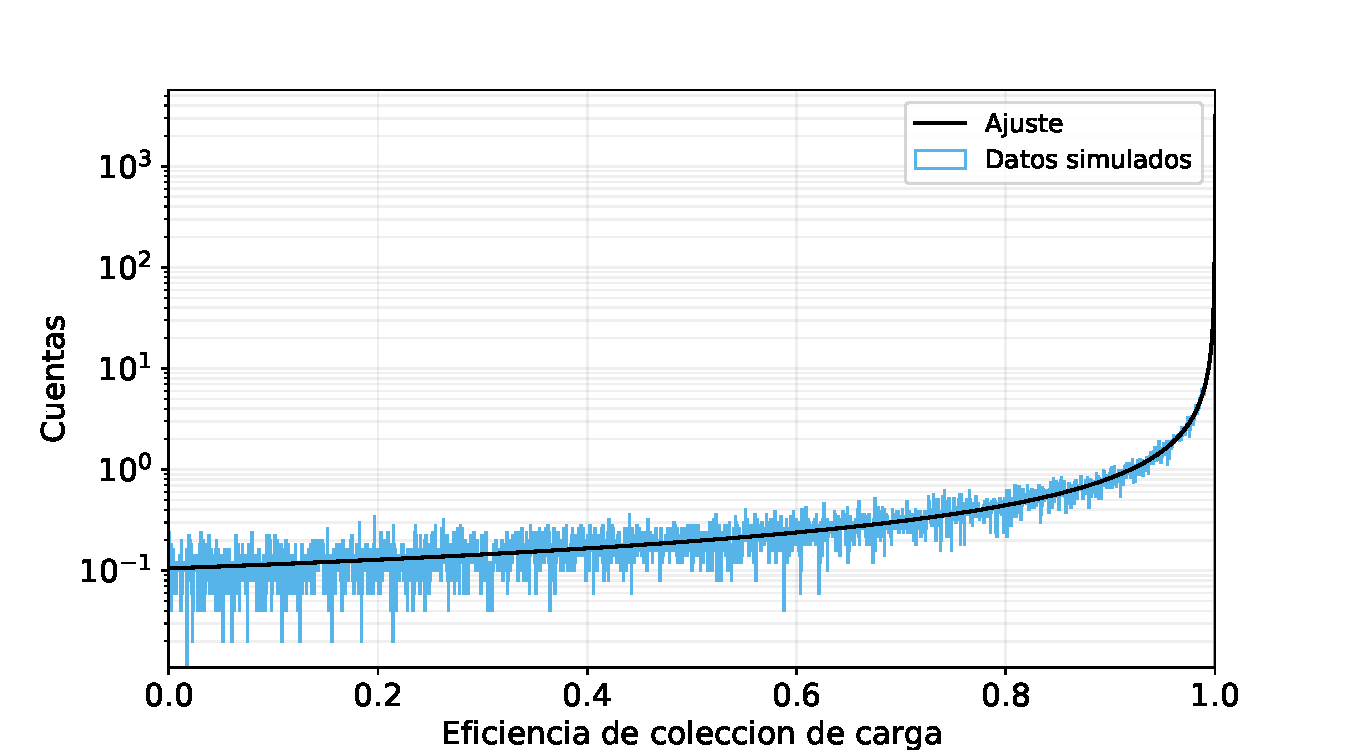
\includegraphics[scale=0.5]{Figs/BetaDistyAjuste.pdf}
    \caption{Distribución de la eficiencia de colección de carga obtenida de una simulación \textit{toy} Monte-Carlo (histograma) y su ajuste con el modelo descripto (trazo continuo).}
    \label{fig:BetaDistyAjuste}
\end{figure}

Sin embargo, para terminar de modelar todos los efectos que contribuyen a la dispersión de la carga generada por ionización en el material, hay que considerar que, además de los efectos anteriores, para una dada energía no siempre se producirán la misma cantidad de carga, efecto descripto por el factor de Fano. Dado que cada proceso de ionización puede considerarse como un experimento de Bernoulli, una sucesión de interacciones puede pensarse como un fenómeno binomial. Cuando la esperanza de dicha distribución es alta (mayor a $100$ para los casos de uso en este trabajo), el límite gaussiano dado por el teorema central del límite se cumple en excelente aproximación. Con lo cual, la distribución de carga para los eventos de interés puede modelarse sin perder precisión con una distribución gaussiana de la siguiente forma
\begin{equation*}
    f_{Q_{i}}(q_{i}) = 
    \frac{1}{\sqrt{2\pi \sigma^{2}}}\,
    \exp
        \left[
            -\frac{1}{2}
            \left(
                \frac{q_{i} - \mu}{\sigma}
            \right)^{2}
        \right]
\end{equation*}
donde $q_{i}$ es la cantidad de carga inicial ionizada. Para agregar esta última contribución al modelado del fenómeno, combinando todas las contribuciones, es necesario realizar la convolución de ambas densidades: la densidad de probabilidad de colectar carga dada una distancia de penetración $z$ y la densidad de probabilidad de generar carga dada una energía inicial. Entonces, se escribe la probabilidad conjunta de ambas como
\begin{equation*}
    f_{Q_{i} \times E_{ff}} (q_{i}, \varepsilon)
    \equiv f_{Q_{i}}(q_{i}) f_{E_{ff}}(\varepsilon)
    =
    \frac{1}{\sqrt{2\pi \sigma^{2}}}
    \exp
        \left[
            -\frac{1}{2}
            \left(
                \frac{q_{i} - \mu}{\sigma}
            \right)^{2}
        \right]
    \beta(1-\varepsilon)^{\beta - 1}
\end{equation*}
Se busca obtener una nueva función densidad $f_{Q_{f}\times E_{ff}}$ para la carga $q_{f}$ que logra escapar de la región de PCC, sin embargo la expresión anterior está escrita en función de la carga ionizada inicial, $q_{i}$. Notando que existe una relación funcional entre ambas que se obtiene a partir de la eficiencia $\varepsilon$ como
\begin{equation*}
    \varepsilon = \frac{q_{f}}{q_{i}}
    \Longrightarrow
    q_{f} = q_{f}(q_{i}),
\end{equation*}
se puede realizar un cambio de variables para obtener la nueva función densidad, siempre y cuando la nueva y la vieja cumplan que
\begin{equation*}
    f_{Q_{f}\times E_{ff}}(q_{f}, \varepsilon)\,dq_{f} =
    f_{Q_{i}\times E_{ff}}(q_{i}, \varepsilon)\,dq_{i}
\end{equation*}
de donde puede obtenerse una expresión para $f_{Q_{f}\times E_{ff}}$ y que escribiendo explícitamente $f_{Q_{i}\times E_{ff}}$ resulta de la forma
\begin{equation*}
    f_{Q_{f}\times E_{ff}}(q_{f}, \varepsilon)
    = 
    \frac{1}{\sqrt{2\pi \sigma^{2}}}
    \exp
        \left[
            -\frac{1}{2}
            \left(
                \frac{q_{i} - \mu}{\sigma}
            \right)^{2}
        \right]
    \beta(1-\varepsilon)^{\beta - 1}
    \left|
        \frac{dq_{i}}{dq_{f}}
    \right|
\end{equation*}
donde se ha agregado un módulo al Jacobiano para asegurar la positividad, sin embargo en este caso en particular no resultará necesario. 

Como $q_{i} = q_{f}/\varepsilon$, y la eficiencia $\varepsilon > 0$, en particular $\varepsilon \in (0, 1]$ entonces se tiene que 
\begin{equation*}
    \left|
        \frac{dq_{i}}{dq_{f}}
    \right|
        = 
    \left|
        \frac{d}{dq_{f}}
        \left(
            \frac{q_{f}}{\varepsilon}
        \right)
    \right|
        = 
        \frac{1}{\varepsilon}
\end{equation*}
reemplazando esto último y acomodando términos se obtiene la función densidad de probabilidad conjunta como
\begin{equation*}
    f_{Q_{f}\times E_{ff}}(q_{f}, \varepsilon)
    = 
    \frac{1}{\sqrt{2\pi \sigma^{2}\varepsilon^{2}}}
    \exp
        \left[
            -\frac{1}{2}
            \left(
                \frac{q_{f} - \varepsilon\mu}{\varepsilon\sigma}
            \right)^{2}
        \right]
    \beta(1-\varepsilon)^{\beta - 1}
\end{equation*}
finalmente, integrando respecto de $\varepsilon$ para obtener la función densidad de probabilidad de $q_{f}$ se llega a la expresión final del modelo,
\begin{equation}
    f_{Q_{f}}(q_{f}) = 
    \int\limits_{0}^{1}
    \frac{\beta(1-\varepsilon)^{\beta - 1}}{\sqrt{2\pi \sigma^{2}\varepsilon^{2}}}
    \exp
        \left[
            -\frac{1}{2}
            \left(
                \frac{q_{f} - \varepsilon\mu}{\sigma\varepsilon}
            \right)^{2}
        \right]\,
    d\varepsilon
    \label{ec:DistribucionFinal}
\end{equation}
el cual fue específicamente construido describir los efectos del factor de Fano y la colección parcial de carga actuando conjuntamente. Por otro lado, al no existir una expresión analítica para la solución de esta integral, fue necesario resolverla numéricamente.

%%%%%%%%%%%%%%%%%%%%%%%%%%%%%%%%%%%%%%%%%%%%%%%%%%%%%%%%%%%%%%%%%%
%%%%%%%%%%%%%%%%%%%%%%%%%%%%%%%%%%%%%%%%%%%%%%%%%%%%%%%%%%%%%%%%
\section{Máxima verosimilitud e incertezas en \texorpdfstring{$\beta$}{beta}\label{sec:MaximaVerosimilitud}}
\noindent La determinación de los parámetros $\mu$, $\sigma$ y $\beta$ del modelo descripto en la sección anterior, se llevó a cabo maximizando la verosimilitud de los datos construida utilizando la distribución \eqref{ec:DistribucionFinal}, presentada en la sección anterior. 

En general, dada una función densidad de probabilidad, la verosimilitud se escribe como la productoria de las densidades evaluadas en los datos medidos, en este caso, la carga colectada $q_{f}$. Es decir
\begin{equation*}
    \Lagr(q_{j}^{f} | \beta, \mu, \sigma) 
    = \prod\limits_{j = 1}^{N}
    f_{Q_{f}}(q_{j}^{f})
\end{equation*}
Dado que se busca maximizar esta expresión, una técnica utilizada para simplificar el cálculo es maximizar su logaritmo natural, de forma que los productos se transforman en sumas y las cuentas pueden resultar más fáciles. Dado que el logaritmo es una función monótonamente creciente, maximizar el logaritmo de la verosimilitud resulta igual que maximizar la verosimilitud. En este sentido, la expresión para el logaritmo natural de la verosimilitud resulta
\begin{equation}
    \ln{(\Lagr(q_{j}^{f}|\beta, \mu, \sigma))}
    = \sum\limits_{j = 1}^{N}
    \ln{
        \left\{
            \int\limits_{0}^{1}
            \frac{\beta(1-\varepsilon)^{\beta - 1}}{\sqrt{2\pi \sigma^{2}\varepsilon^{2}}}
            \exp
                \left[
                    -\frac{1}{2}
                    \left(
                        \frac{q_{j}^{f} - \varepsilon\mu}{\sigma\varepsilon}
                    \right)^{2}
                \right]\,
            d\varepsilon
        \right\}
    }.
\end{equation}
Resolviendo numéricamente la integral, la técnica consiste en mover los parámetro $\beta$, $\mu$ y $\sigma$ hasta obtener el valor máximo del logaritmo de la verosimilitud. 

Por otro lado, debido a que el efecto que introduce en las mediciones la colección parcial de carga es pequeño, se espera que la estadística sea baja en las colas de los picos. Es por esa razón que la sensibilidad del ajuste al parámetro $\beta$ es menor que la que se encuentra con $\mu$ y $\sigma$, que se nutren de toda la estadística del pico. Para llevar adelante un análisis más robusto de la incerteza del parámetro $\beta$ se hizo uso de otras herramientas de cálculo. Para ello se calculó el logaritmo de la verosimilitud frente a un un barrido en este parámetro optimizando en cada paso los valores de $\mu$ y $\sigma$. Se busca luego el intervalo de confianza de la verosimilitud de $68.3\,\%$ de probabilidad que contenga al parámetro $\beta$. El $\hat{\beta}$ será aquél que maximiza el valor del logaritmo de verosimilitud siendo su intervalo de confianza el conformado por $\beta_{min}$ y $\beta_{max}$ tales que el logaritmo de la verosimilitud tome el valor de su máximo menos 1/2, es decir, el intervalo está conformado por aquellos valores de $\beta$ que cumplan la siguiente condición:
\begin{equation*}
    \left\{
        \beta\ \in\ \mathbb{R}\ /\ 
        \ln{(\Lagr(\hat{\beta}))}
        -
        \ln{
            \left(
                \Lagr(\beta)
            \right)
            }
        < 1/2
    \right\}
\end{equation*}
Los $\beta$ donde la recta y la parábola se tocan corresponden a los límites izquierdo $\beta_{min}$ y derecho $\beta_{max}$ del intervalo de $68.3\,\%$ deseado\cite{Frodesen}.

%%%%%%%%%%%%%%%%%%%%%%%%%%%%%%%%%%%%%%%%%%%%%%%%%%%%%%%%%%%%%%%%%%%%
%%%%%%%%%%%%%%%%%%%%%%%%%%%%%%%%%%%%%%%%%%%%%%%%%%%%%%%%%%%%%%%%%%

\section{Características del modelo}

\noindent Utilizar este modelo para ajustar los picos de los histogramas de carga tiene la ventaja de que los parámetros que se obtienen del ajuste, como el valor medio $\mu$ y la dispersión $\sigma$, son aquellos valores que se obtendrían si la colección parcial de carga fuera totalmente nula. Es decir, este modelo logra obtener estas magnitudes disociando totalmente el efecto de la PCC. A su vez, también se obtiene el parámetro $\beta$, el cual se definió como la relación entre $\tau_{\scaleto{CCE}{4pt}}$ y $\tau_{\scaleto{X}{4pt}}$, donde el primero es un parámetro intrínseco del detector y, por ende, está fijo, mientras que el segundo es una magnitud que varía dependiendo de la energía incidente y del material. Cabe aclarar que para modelar un posible fondo proveniente de la PCC de picos más a la derecha de los de interés se agrega un término constante al ajuste. Este término no se ajusta junto con el resto de los datos, sino que se ajusta previamente usando solo el fondo a derecha de los picos.

Vale mencionar que este modelo se enfoca en capturar el efecto que provoca la colección parcial de carga en los picos de los histogramas, e ignora la dispersión por efecto Compton o la generación de pares. Esto se debe a que en las escalas de energía en las que se trabajó, los efectos de estos fenómenos son despreciables o, más aún, imposibles para el caso de generación de pares. 
\begin{figure}[h]
    \centering
        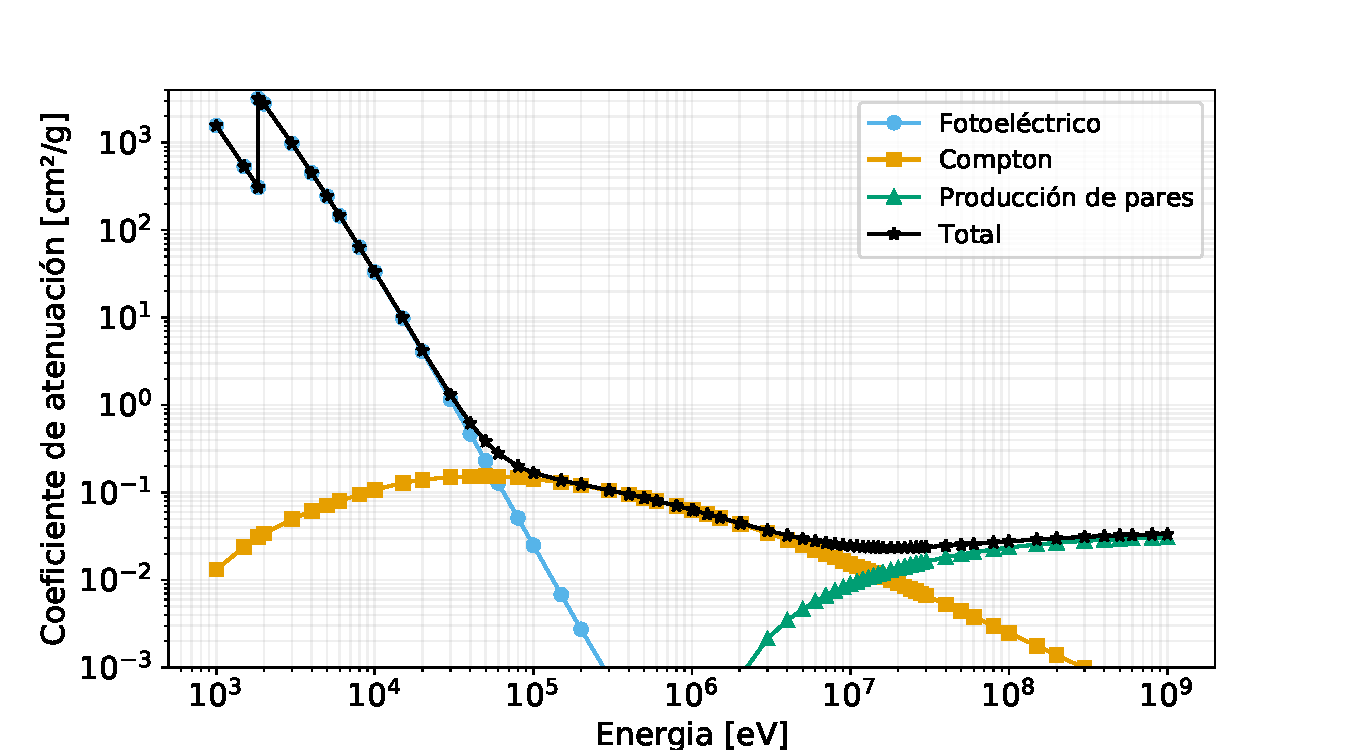
\includegraphics[scale=0.5]{Figs/FotoelectricoComptonPares_enSilicio.pdf}
    \caption{Diferentes contribuciones al coeficiente de atenuación del Silicio. Se observa que el efecto fotoeléctrico es la contribución preponderante en los órdenes de energía estudiados en este trabajo.}
    \label{fig:FotoelectricoComptonPares}
\end{figure}
En el gráfico de la Figura \ref{fig:FotoelectricoComptonPares} se encuentran las curvas de los coeficientes de atenuación para el silicio dependiendo del tipo de proceso de dispersión, obtenidas del \textit{National Institute of Standards and Technology}\cite{FotoComptPar}, como ser, el efecto fotoeléctrico, el efecto Compton, la generación de pares y la suma de los tres efectos. Se observa de la Figura \ref{fig:FotoelectricoComptonPares} que para energías menores a los $1000\,\si{eV}$ la contribución del efecto Compton es totalmente despreciable frente a la del efecto fotoeléctrico, la cual domina en todo el rango de energías de estudiado en este trabajo.

Resulta importante notar que, debido a que la longitud de atenuación $\tau_{\scaleto{X}{4pt}}$ depende de la energía del fotón incidente (entre otros), para el caso de los rayos $X$ del flúor cuya energía es menor a la de los rayos $X$ del aluminio, la longitud de atenuación es menor. Por otro lado, como $\tau_{\scaleto{CCE}{4pt}}$ es una característica del detector y no depende de ningún parámetro, y como $\beta = \tau_{\scaleto{CCE}{4pt}}/\tau_{\scaleto{X}{4pt}}$, entonces se espera que el valor de $\beta$ sea mucho mayor en el caso del flúor respecto del aluminio. Con lo cual, el efecto de la colección parcial de carga debería ser más pronunciado en esos picos. Esto implica que debería poder apreciarse colas más pronunciadas hacia bajas energías en los espectros obtenidos con $X$ del flúor que aquellos correspondientes al aluminio.

%\indent Si el detector fuera perfecto, el factor de Fano existiría igual. Este no es un problema del detector, viene del proceso de interacción en sí mismo que a la larga es un fenómeno binomial. Sin embargo, lo que sí es un problema del detector es la PCC. Un fotón interactuando con materia es un experimento Bernoulli, una serie de procesos de interacción es un fenómeno binomial y, en consecuencia, en el límite de probabilidades pequeñas y gran número de repeticiones, de Poisson. Por lo tanto, cuán lejos llega es una variable aleatoria con distribución exponencia (La distancia entre dos eventos de poisson es exponencial). Si uno quiere saber cuál es la probabilidad de que un fotón penetre una dada distancia, hay que hacer
%\begin{equation*}
%    e^{-\frac{d}{\tau}}
%\end{equation*}
%con $\tau$ es la attenuation length. La eficiencia de colección de carga viene dada por 
%\begin{equation*}
%    E_{ff}(z) = 1 - e^{-\frac{z}{\tau_{\scaleto{CEE}{2pt}}}}
%\end{equation*}
%que quiere decir que si la interacción se realizó para un dado $z_{0}$, entonces por ejemplo el $70\%$ de la carga logró ser colectada. Para $Z_{0}$ muy chico, la eficiencia es muy chica, para $z_{0}$ creciente, la eficiencia es creciente.

%Dada la variable aleatoria: Longitud penetrada hasta interactuar, tiene una distribución exponencial. Dada una energía fija, la longitud que recorre hasta interactuar no es siempre la misma, hay una aleatoria inherente. La distribución de probabilidades de este experimento es exponencial. Si por ejemplo la probabilidad de interactuar en los primeros $3\,\si{\mu m}$ es del $50\%$, la probabilidad de interactuar recién luego de recorridos $80\,\si{\mu m}$ es $10^{-14}$. Esta variable aleatoria se inyecta dentro de la función $E_{ff}(z)$: Función a la que le digo hasta donde llegó la partícula antes de interactuar y devuelve con qué eficiencia colectó la carga.

%Se tiene la energía del fotón, se genera un evento aleatorio con distribución exponencial $z_{0}$ que dice qué distancia penetró el fotón antes de interactuar. Esa realización se usa como argumento de $E_{ff}(z) \longrightarrow E_{ff}(z_{0})$. Ese cambio de variables da como resultado 
%\begin{equation*}
%    f_{E_{ff}}(z) = \beta (1 - \varepsilon)^{\beta - 1}
%\end{equation*}
%donde $\beta = \frac{\tau_{\scaleto{CCE}{3pt}}}{\tau_{\scaleto{X}{3pt}}}$. La probabilidad de recuperar la carga de un fotón de una dada energía sigue esa distribución.

%Todavía no entró el Fano. A esto hay que agregarle que además de haber una distribución de carga para la profundidad, además de haber una función que dice cuánta carga se logra colectar con esa profundidad, hay otra variable aleatoria que es cuántos electrones se ionizan cuando se interactúa, que viene de una poissoniana, pero en el límite se puede pensar como una gaussiana. Entonces, a la función anterior hay que convolucionarla con una gaussiana. El efecto de convolucionar una gaussiana con esta distribución es añadirle una cola del lado izquierdo a la gaussiana. De hacer esa convolución se obtiene
%\begin{equation*}
%     f_{Q_{f}}(q_{f}) = 
%     \int\limits_{0}^{1}
%     \frac{\beta}{\sqrt{2\pi \sigma^{2}}\varepsilon}
%     \exp[%
%     -\frac{(q_{f}-\varepsilon\mu)^{2}}{2\sigma^{2}\varepsilon^{2}}
%     ](1-\varepsilon)^{\beta - 1}
%     d\varepsilon
% \end{equation*}
%La cola que aparece a la izquierda es culpa de la PCC, debido a que hay eventos con menor carga generada debido a este fenómeno de recombinación para los eventos que suceden en los primeros micrones del detector. Del lado derecho no hay nada porque no hay un fenómeno que genere más carga de la que el proceso de ionización puede generar.
%%%%%%%%%%%%%%%%%%%%%%%%%%%%%%%%%%%%%%%%%%%%%%%%%%%%%%%%%%%%%%%%%%
%%%%%%%%%%%%%%%%%%%%%%%%%%%%%%%%%%%%%%%%%%%%%%%%%%%%%%%%%%%%%%%%%%
